\chapter{Einleitung}\label{chap:intro}
\section{Motivation}

\section{Scala}
Wir haben uns entschieden, das Programm in Scala zu schreiben, einer Sprache, die bereits schon im Jahr 2001 von Martin Odersky entwickelt wurde, jedoch erst seit kurzem einen großen Bekanntheitsgrad erlangt hat. Grund dafür ist der Hype um die sogenannte \texttt{funktionale Programmierung} und das Bedürfnis, Anwendungen nebenläufig zu entwickeln. 
Wir möchten nun zu Beginn die Gründe nennen, warum Scala sich als moderne Programmiersprache anbietet, die sogar von Javas Hauptentwickler James Gosling als bevorzugte Java-Alternative betitelt wurde \footnote{\url{http://www.adam-bien.com/roller/abien/entry/java_net_javaone_which_programming}}.

\subsection{Laufzeit-Umgebung}
Scala ist wie Java eine Programmiersprache, die zu Bytecode kompiliert wird. Dieser Bytecode wird dann von der \textit{Java Virtual Machine} (\texttt{JVM}) benutzt um daraus Maschinencode zu erstellen. Die JVM ist mittlerweile auf sehr vielen Rechnern installiert und sogar das Android Betriebssystem setzt auf eine Variante der \texttt{JVM} (\texttt{Dalvik}).

Die JVM hat den großen Vorteil, dass sie mittlerweile seit 20 Jahren aktiv entwickelt wird und die gesamte Java-Umgebung besonders im Enterprise Bereich eingesetzt wird. Das Resultat ist ein sehr stabiles und vor allem perfomantes System, das aus dem heutigen IT-Markt nicht mehr wegzudenken ist. 

\subsection{Bibliotheken}
Scala wird also nicht zu irgendeinem Bytecode kompiliert, sondern zu Java-Bytecode, um genau zu sein. Dies hat den großen Vorteil, dass man neben der JVM-Unterstützung auch auf etablierte Java Bibliotheken zugreifen kann. Beispielsweise ist der Einsatz von Google GSON\footnote{Link zu der Projektseite von Google GSON: \url{https://github.com/google/gson}}, das das Serialisieren von Objekten in JSON und zurück ermöglicht, über Scala so möglich, wie über Java.

So ist es dann auch kaum überraschend, dass der Einsatz von den üblichen Java Bibliotheken in Scala möglich ist. Ein Beispiel ist \texttt{JavaFX}, welches seit Java 8 Teil des \textit{Java Development Kit} (\textit{JDK}) ist.

\subsection{JavaFX und ScalaFX}
\texttt{JavaFX 8} ist der offzielle Nachfolger von \texttt{Swing}. Zu Beginn sollte es eine Scriptssprache werden, jedoch wurde dieser Fokus mit Version 2 aufgegeben und JavaFX wurde zu der GUI Bibliothek, wie man sie heute nutzt. In der aktuellen Version 8 (welcher der direkte Nachfolger von Version 2 ist und wegen der Einbindung in das JDK 8 diesen Versionssprung vollzogen hat), wurde die Bibliothek um wichtige Komponenten erweitert und bietet die folgendenden Vorteile: 

\begin{description}
\item[Scene Graph] JavaFX ist besonders leicht zu entwickeln, da es auf den \texttt{Scene Graph} setzt. Der Scene Graph ist eine Baumstruktur, bei der die Elemente hierachisch angeordnet werden. Elemente im Scene Graph sind vom Type \texttt{Node} ~\cite{ProJavaFX8}. Wenn man also beispielsweise einen Button auf der Bildfläche platzieren möchte, dann hat man ein Button Objekt, welches von \texttt{Node} erbt

\begin{figure}[!htb]
    \centering
      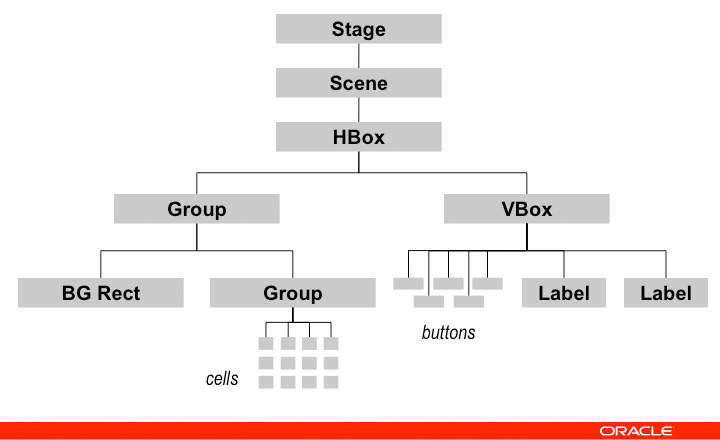
\includegraphics[width=0.75\linewidth]{scene-graph}
    \caption{Darstellung der Baumstruktur im Scene Graph}
    \label{fig:scene-graph}
\end{figure}

Ein Vorteil ist, dass man so Objekte gruppieren kann und dadurch Operationen auf der Gruppe ausführen kann. So wird bei einer Verschiebe-Operation (auch \texttt{Translation} genannt) jedes Element in der Gruppe verschoben, was den Code lesbarer und wartbarer macht.\
Außerdem ist somit eine zum Eltern Element relative Positionierung möglich.

%TODO: Section FXML einbinden
\item[Klares MVC] Bei JavaFX wird das Konzept für das Design in einer separaten Datei, einer \texttt{FXML} Datei geführt. So muss man das Layout nicht im Code generieren. Im Abschnitt zu FXML~\ref{sec:fxml} wird dies ausführlicher beschrieben.

\end{description}

\subsection{FXML}\label{sec:fxml}

\section{Ziele \& Fragen}
\section{Methodische Vorgehensweise}